\chapter{Robot Operating System - ROS}\label{cap:ros}

\begin{citacao}
``O Robot Operating System (ROS) é um conjunto de bibliotecas de software e ferramentas que te auxiliam na construção de aplicações em robótica. De drivers ao estado da arte de algoritmos, e com poderosas ferramentas de desenvolvimento, ROS tem o que você precisa para seu próximo projeto de robótica. E tudo é open source~\cite{Ros}''    
\end{citacao}

O ROS foi idealizado com o objetivo de ser um ambiente completo, de código aberto, para elaboração de sistemas robóticos. Largamente aceito e amplamente utilizado atualmente, os desenvolvedores se beneficiam da alta qualidade de código proporcionado pelo grande número de usuários e plataformas que aproveitam-se do ROS em seus projetos~\cite{RosIntro}. Uma ampla variedade de sensores e atuadores empregados na robótica também seguem essa tendência e oferecem suporte ao ROS através de seus drivers. O ROS fornece abstração de hardware, controle de baixo nível para dispositivos, funcionalidades e bibliotecas de uso comum, passagem de mensagens entre processos e gerenciamento de pacotes~\cite{rosEfetiveProgram}. Por esses motivos, o ROS é conhecido como um meta sistema operacional para robôs. Neste capítulo será apresentado o ROS e as vantagens do seu uso na concepção de novas plataformas robóticas.

A cada ano o ROS vem se consolidando como o framework padrão para o desenvolvimento de novos projetos de robótica, apesar de já possuir este status, o ROS possui uma história relativamente curta. O ROS teve início no Laboratório de Inteligência Artificial de Standord e em 2007 a companhia Willow Garage assumiu o seu desenvolvimento. A Willow Garage é uma empresa que desenvolve robôs pessoais e de serviços. Ela também é responsável pelo desenvolvimento de suporte a \textit{Point Cloud Library (PCL)}, que é uma biblioteca de software largamente usada para processamento de nuvens de pontos. Em Janeiro de 2010 a primeira versão do ROS foi lançada, desde então muitas outras versões foram lançadas. O ROS está sob as licenças BSD 3-Clause e Apache 2.0, que permite qualquer um modificar, reusar e distribuir códigos ROS~\cite{rosPYO}. Atualmente o ROS se encontra com uma versão estável do ROS2 e o ROS uma tem seu fim marcada para maio de 2015.



\section{Um sistema operacional para robôs}

De forma simplificada um sistema operacional tem como objetivo gerenciar os recursos do sistema computacional, ele atua como uma ponte entre esses recursos e o seu usuário, ou seja, o sistema operacional se faz necessário para disponibilizar às aplicações os recursos funcionais do sistema de forma padronizada, se tornando uma verdadeira camada de abstração entre os programas e o hardware. Windows, Ubuntu, para computadores pessoais e Android para smartphones, são exemplos de sistemas operacionais populares.

A comunidade da robótica em todo mundo tem feito grande progresso nos últimos anos. Hardware confiáveis e com menor custo têm sido ofertados em um nível nunca encontrado no passado, desde robôs móveis terrestres, passando por drones e até mesmo robôs humanóides estão disponíveis no mercado com relativa facilidade. O que pode ser até mais impressionante, a comunidade também tem desenvolvido algoritmos que permitem que estes robôs possuam um nível crescente de autonomia. Apesar desse rápido progresso, o desenvolvimento de robôs ainda representam um desafio para os desenvolvedores de softwares e grande parte desse desafio se deve a falta de padronização de um software específico para robótica, ou até mesmo um sistema operacional dedicado para robôs, como podemos encontrar em outros nichos, como os PCs e smartphones e o ROS tenta preencher essa lacuna.

O nome ROS vem da abreviação de Robot Operating System, mas seria o ROS um sistema operacional para robôs? Ele fornece abstração de hardware, controle de baixo nível para dispositivos, implementações de funcionalidades de uso comum, troca de mensagens entre processos, até um sistema de gerenciamento de pacotes. Além destas características o ROS está equipado com bibliotecas e ferramentas para escrever, compilar e rodar seus códigos~\cite{RosIntro}.

Apesar de todos os atributos que o caracterizam como um sistema operacional, o ROS não é um sistema operacional convencional, por ainda precisar rodar em um outro sistema operacional previamente instalado, o que faz com que o ROS seja conhecido como um meta-sistema operacional. Antes de ter o ROS em execução no robô é necessário instalar um sistema operacional, como por exemplo o Ubuntu. Com a distribuição Linux rodando é possível executar a instalação completa do ROS, sendo assim, todos os recursos fornecidos por um sistema operacional convencional podem ser utilizados pelo ROS, como sistema de gerenciamento de processos, sistema de arquivos, interface do usuário, compiladores entre outros. 

Para complementar esses recursos básicos do sistema operacional o ROS fornece funcionalidades específicas para o uso na robótica, tal como libraries para transmissão e recepção de dados para uma variedade de hardwares comumente utilizados em sistemas robóticos. Esse tipo de software é conhecido como middleware ou framework. Como pode ser visto na Figura~\ref{fig:rosmeta}, o ROS é o sistema auxiliar para controlar atuadores e sensores, com um nível de abstração de hardware dando suporte para o desenvolvimento de novas aplicações de robótica em sistemas operacionais convencionais.

\begin{figure}[ht]
	\caption{ROS um meta-sistema operacional}
	\begin{center}
		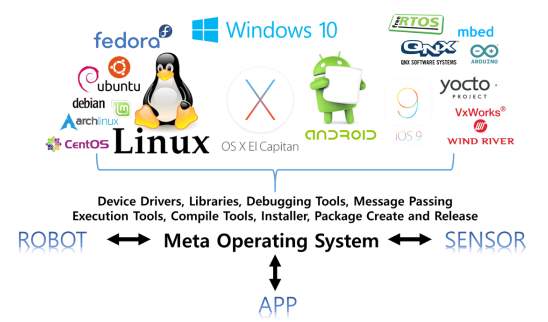
\includegraphics[scale=0.6]{imagens/metaOS.png}\\
		{\small \textbf{Fonte:} \citeonline{rosPYO}}
    \end{center}\label{fig:rosmeta}
\end{figure}



\section{Vantagens do ROS}
Até agora descrevemos o ROS como uma ferramenta ideal para o desenvolvimento de novos projetos de robótica, apesar disto, aprender a usar um novo framework é uma atividade árdua, principalmente um tão abrangente e complexo como o ROS. Esse tipo de questão deve ser levada em consideração na escolha das ferramentas no inicio de um novo projeto. 

O objetivo do ROS não é ser um framework com o maior número de recursos, seu principal objetivo é oferecer o máximo de reuso de softwares usados no desenvolvimento de novos robôs. O ROS é um framework de computação distribuída, isso que dizer que os seus processos podem ser projetados individualmente e podem ser integrados ao sistema livremente e em tempo de execução. Estes processos podem ser agrupados em pacotes, facilitando o compartilhamento e a sua distribuição. Outra iniciativa para incentivar a colaboração e o compartilhamento de código são os repositórios oficiais do ROS, que estão disponíveis de forma livre. 

A seguir serão listadas algumas características que incentivam a colaboração da comunidade e são responsáveis pelo sucesso do ROS\@:

\begin{itemize}
    \item\textbf{Recursos Nativos:} O ROS oferece, de forma nativa, muitos recursos prontos, testados e validados pela comunidade. Podemos citar como exemplos o \textit{Simultaneous Localization and Mapping (SLAM)} e o \textit{Adaptive Monte Carlo Localization (AMCL)} que são usados para navegação autônoma de plataformas robóticas móveis, outro pacote oferecido pelo ROS é o MoveIt,pacote usado para planejamento de movimento de manipuladores. Estes recursos podem ser usados sem nenhum problema e são altamente configuráveis, podendo ser adaptados em vários modelos de robôs e atender a inúmeras aplicações. 

    \item\textbf{Ferramentas de desenvolvimento:} O ROS é disponibilizado com uma grande quantidade de ferramentas para debugging, visualização, incluindo ferramentas para simulação. Algumas das ferramentas open source mais poderosas para visualização, debugging e  simulação, respectivamente, rqt\underline{ }gui, RViz e Gazebo, são nativas do ambiente ROS\@.
    
    
    \item\textbf{Suporte sensores e atuadores:} Muitos dos sensores e atuadores usados na robótica já são suportados pelo ROS e o número de dispositivos compatíveis aumenta a cada ano. Algumas companhias se beneficiam pelo fato de muitos desses dispositivos fazerem uso de hardware aberto e o software existente também pode ser reutilizado a custo zero. Fazendo com que o processo de desenvolvimento de novos hardware periféricos usados na robótica também acelere. Sensores como Velodyne-LIDAR, Laser scanners e atuadores como os servos Dynamixel, podem ser integrados ao ROS sem nenhum impedimento.
    
    \item\textbf{Múltiplas linguagens:} O framework ROS pode ser programado em algumas linguagens de programação modernas. Pdemos escrever código eficientes em C ou C++ e outra aplicação ser escrita em python. O ROS possui bibliotecas clientes para C/C++, Python, Java e Lisp. Este tipo de flexibilidade não é comum em outros frameworks.
    
\end{itemize}




\subsection{Computacão distribuida}
Grande parte de robôs modernos possuem diferentes unidades de processamentos, que podem estar localizados em diferentes computadores. Desde sensores microprocessados até mesmo controles específicos para motores, podem possuir suas próprias unidades computacionais. Mesmo possuindo apenas um computador, dividir o processamento em processos individuais específicos para cada função e fazer com que eles trabalhem em conjunto para se afim de resolverem um problema maior é uma excelente abordagem para a arquitetura de robôs modernos. Além disso, múltiplos robôs podem trabalhar de forma colaborativa dividindo atividades entre eles, ou até mesmo interagindo com seres humanos que poderiam enviar comandos através de um computador ou celular. Em todos estes casos é necessário a comunicação entre processos, que podem ou não estarem no mesmo computador. 

O ROS é um Inter-process communication framework e de fato ele usa uma rede TCP/IP para realizar essa comunicação entre processos. Ele usa sockets TCP/IP para transportar dados entre os processos. Esta abordagem proporciona grande flexibilidade na troca de mensagem, processos podem se comunicar com outros mesmo se eles não estiverem na mesma máquina, ou até mesmo em robôs separados, bastando para isso, todas as máquinas que compartilham processos estarem na mesma rede. Isso faz com que até mesmo processos rodando na internet possam participar da comunicação e realizar uma parte do processamento de um robô.


\subsection{Reuso de Software}
O uso do ROS pode diminuir a necessidade de implementar algoritmos que já foram testados e validados por outros pesquisadores. Algoritmos de navegação, planejamento de rotas, mapeamento entre outro, são usados em diferentes projetos, e o ROS permite que estes algoritmos sejam reaproveitados de duas maneiras possíveis:

\begin{itemize}
    \item \textbf{Pacotes padrões:} São pacotes de softwares de importantes algoritmos usados na robótica ou mesmo drivers de dispositivos comuns na robótica, que já foram implementados e testados.

    \item \textbf{Interface de troca de mensagens:} A interface utilizada pelo ROS vem se tornando um padrão na comunicação entre processos em robôs.
\end{itemize}


Nos repositórios oficiais do ROS estão disponíveis centenas de pacotes públicos que utilizam a interface de troca de mensagens padronizada do ROS possibilitando uma redução significativa do esforço necessário para o desenvolvimento de uma lógica para integrar estes pacotes ao seu sistema. Logo desenvolvedores que usam o ROS podem concentrar mais tempo e esforços no desenvolvimento de suas novas ideias, aproveitando algoritmos consolidados dos repositórios oficiais do ROS, sem a necessidade de reescrevê-los para adaptá-los ao seu projeto.


\subsection{Testes Rápidos}


\section{Sistemas de aquivos}
Como era de se esperar de um sistema operacional, o ROS também possui um sistema de arquivos padronizado. É de extrema importância para o desenvolvimento de novas aplicações conhecer a organização dessa estrutura de arquivos. A Figura~\ref{fig:rosfile} apresenta um diagrama de blocos do sistema de arquivo do ROS\@.

\begin{figure}[ht]
	\caption{Sistema de arquivos ROS}
	\begin{center}
		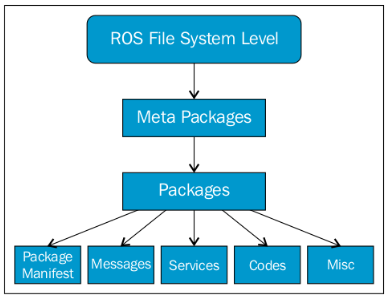
\includegraphics[scale=0.7]{imagens/fileSiystem.png}\\
		{\small \textbf{Fonte:} \citeonline{rosMastering}}
    \end{center}\label{fig:rosfile}
\end{figure}

A seguir são apresentados a definição de cada bloco da estrutura de arquivos do ROS\@:
\begin{itemize}
    \item \textbf{Pacotes:} Pacotes são a unidade de software principal do ROS\@. Um pacote pode conter nós, dependências, bibliotecas, datasets, arquivos de configuração, ou qualquer coisa que seja útil organizar de forma agrupada~\cite{RosPKG}.

    \item \textbf{Manifesto do pacote:} O arquivo package.xml é conhecido como manifesto do pacote, ele fornece os metadados a respeito do pacotes, incluindo nome, versão, descrição, licença, dependências e outras informações. Os padrões do package.xml são definidos no REP-0127.
    
    \item \textbf{Metapackages:} Metapackages são pacotes especializados que serve apenas como representante de um grupo de outros pacotes relacionados entre si.
    
    \item \textbf{Meta packages manifest:} O manifesto de um metapackage é semelhante ao manifesto de um pacote comum, a diferença entre eles é que no manifesto devemos incluir as dependências encontradas no mesmo repositório do meta package
    
    \item \textbf{Message (msg) types:} É o arquivo de descrição de um tipo de mensagem, é armazenado no diretório my\underline{ }package/msg/MyMessageType.msg e define toda a estrutura de dados enviados a partir deste tipo de mensagem.
    
    \item \textbf{Service (srv) types:} É o arquivo de descrição de um tipo de mensagem, é armazenado no diretório my\underline{ }package/srv/MyServiceType.msg e define toda a estrutura de dados enviados a partir deste tipo de serviço.
    
    \item \textbf{Repositórios:} Pacotes ROS são compartilhados usando algum tipo de Version Control System (VCS), como o gti. Cada repositório pode conter apenas um pacote ou um metapackage 
\end{itemize}


\subsection{Pacotes ROS}

A unidade básica para configuração do software no ROS é conhecida como pacote, isso quer dizer que todas as aplicações desenvolvidas para ROS são estruturadas como um pacote. Na Figura XX podemos ter uma visão da estrutura típica de uma pacote ROS

\begin{figure}[ht]
	\caption{Estrutura típica de um pacote ROS ROS}
	\begin{center}
		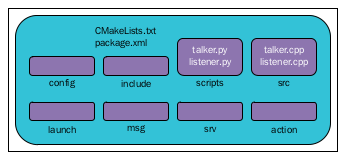
\includegraphics[scale=0.8]{imagens/rospackagestruture.png}\\
		{\small \textbf{Fonte:} \citeonline{rosMastering}}
    \end{center}\label{fig:rospacotestrut}
\end{figure}

Nos pacotes estão contidos um ou mais nós, como são chamadas as unidades de processamento no ROS, ou podem incluir arquivos de configuração para a execução de nós de outros pacotes. Existem milhares de pacotes ROS oficiais e uma quantidade ainda maior de pacotes desenvolvidos por seus usuários. 

Cada metapackage possui um arquivo chamado package.xml, este arquivo é responsável por reunir informações importantes sobre o pacote, nele podemos encontrar o nome do pacote, seu autor, dependências e licença de uso. O sistema de compilação do ROS é o Catkin, ele usa o CMake e o arquivo CMakeLists.txt que deve estar dentro da pasta de cada pacote com as suas instruções de compilação. 

Os pacotes são as menores unidades que podem ser compiladas no ROS, são também  a maneira com que podemos organizar o software para ser lançado. No caso dos pacotes oficiais do ROS, por exemplo, existe um pacote Debian, que são os pacotes utilizados pelo Ubuntu, para cada pacote ROS. Apesar do conceito ser semelhante, e mesmo que ao instalar um pacote Debian, você possa incluí-lo à sua lista de pacotes ao ROS instalado no sistema, os pacotes debian e ROS não são equivalentes. 

A principal função dos pacotes é ser uma maneira funcional, de fácil configuração e um caminho descomplicado para possibilitar o reuso de software. De maneira geral o pacotes ROS devem conter funcionalidades suficientes para serem úteis, mas não muito para torná-los muito grande e confuso, tornando seu uso difícil por outro software 



\subsection{Mensagens ROS}


\section{Sistemas computacional ROS Graph level}
entendendo ROS node
ROS TOPIC
ROS master
ROS Parameters
Workspace ROS


\section{Community level- ROS ecosistema}











% No ROS um processo é conhecido como nó, que pode receber e enviar mensagens para se comunicar com outros nós através de uma rede rodando o protocolo TCPROS [3].a busca por sistemas com um grau maior de autonomiaA robótica tem se caracterizádo pelo grande nível de percepção do ambiente e pelos sistemacomplexos de controle do movimentos 

% Com essa distribuição de tarefas através de vários nós podemos criar sistemas cada vez mais complexos, apenas inserindo novos nós na rede, essa rede é gerenciada pelo ROS Master, que é apensas mais um nó do sistema, mas com a função de ser um servidor de nome e serviços para o restante dos nós. Ele identifica os nós na rede, assim todos os nós podem se comunicar com os outros através de conexões peer-to-peer, igura 1. Para desenvolver novas aplicações para o crescente grupo de pacotes ROS, o desenvolvedor deve respeitar os protocolos de comunicação da rede, as bibliotecas do ROS facilitam este trabalho, por já fornecer funções prontas para o desenvolvimento de novos códigos compatíveis e que possam se registrar na rede. Detalhes dos  rotocolos e interno podem ser visto em (ROS, 2011a), (ROS, 2018) e (ROS, 2011b).



% Desenvolver um robô não é algo trivial, atividades que seriam facilmente executadas por nós, seres humnos, como por exemplo, andar de um ponto ao outro de uma sala, do ponto de vista de um robô pode ser um trabalho extremamente árduo. Montar o sistema que possibilite o robô executar as funções pra o qual foi projetado pode facilmente necessitar de um arranjo complexo entre componetes de software e hardware e que pode variar bastante dependendo do ambiente ao qual o robô será exposto. Sendo assim, o desenvolvimento de um sistema robôtico completo necessita de uma conhecimento abrangente e de áreas distintas.  

% Nesse paronama que o ROS foi concebido, com o objetivo de  ser um um ambiente completo para desenvolvimento de sistemas robôticos, facilitando o desenvolvimento com o máximo de reuso de código possibilitando o mínimo de mudanças na adaptação um sistema a um novo ambiente ou até mesmo no desenvolvimento de uma nova plataforma. Atualmente o ROS é um framework bem aceito e amplamente utilizado não apenas na comunidade acadêmica mas também na industria. Desenvolvido originalmente em 2007 no \textit{Stanford Artificial Intelligence Laboratory - SAIL}, a partir de 2008 o ROS foi continuado pela Willow Garage, entretanto em 2012 com a criação da \textit{Open Source Robotics Foundation, Inc. - OSRF} os ROS e projetos parceiros como o Gazebo passaram a ser mantidos pela própria OSRF, que continua o desenvolvimento adicionando novas fancionalidades ao projeto. Além disso muitas instituições de pesquisa adaptaram seus projeto ao ROS, aumentando a cada ano o número de pesquisadores e desenvolvedores trabalhando no aperfeiçoamento do ROS. No site oficial do ROS podemos ver uma lista com diverssas plataformas que utilizam o ROS em seus projetos. http://wiki.ros.org/Robots





% It uses graph architecture with a centralized topology, where processing takes place in nodes that may receive and send messages to communicate with other nodes on the graph net. A node is any process that can read data from a sensor, control an actuator, or run high level, complex robotic or vision algorithms for mapping or navigating autonomously in the
% environment.\cite{rosEfetiveProgram}




% Distributed process: It is programmed in the form of the minimum units of executable processes (nodes), and each process runs independently and exchanges data systematically. Package management: Multiple processes having the same purpose are managed as a package so that it is easy to use and develop, as well as convenient to share, modify, and redistribute. Public repository: Each package is made public to the developer’s preferred public repository (e.g., GitHub) and specifies their license. API: When developing a program that uses ROS, ROS is designed to simply call an API and insert it easily into the code being used. In the source code introduced in each chapter, you will see that ROS programming is not much different from C++ and Python. These characteristics of ROS have allowed users to establish an environment where it is possible to collaborate on robotics software development on a global level. Reusing a code in robot 



